\documentclass[twocolumn,hyperpdf,
amsmath,amssymb,
aps,prd,10pt,
superscriptaddress,nofootinbib,noeprint,preprintnumbers]{revtex4-1}


\usepackage{graphicx}% Include figure files
\usepackage{dcolumn}% Align table columns on decimal point
\usepackage{bm}% bold math
\usepackage{amsmath}
\usepackage{amsfonts}
\usepackage{slashed}
\usepackage{hyperref}
\usepackage{multirow}
\usepackage{soul}
\usepackage{mathtools}
\usepackage{float}
\usepackage{afterpage}
\usepackage{color}


\usepackage{amsmath,amssymb}
\usepackage{graphicx}
\usepackage{bm}
\usepackage{comment} 
\usepackage{subfigure}
\usepackage{array}
\usepackage{multirow} 

\newcommand{\gsim}{\raisebox{-0.7ex}{$\stackrel{\textstyle >}{\sim}$ }}
\newcommand{\lsim}{\raisebox{-0.7ex}{$\stackrel{\textstyle <}{\sim}$ }}
\newcommand{\nn}{\nonumber}

\newcommand{\Erho}{\rm 754(3)(1)(^{19}_{01})-i\,65(2)(1)(^{1}_{3})~MeV}

\newcommand{\raul}{\bf \color{blue}}
\newcommand{\warning}{\bf \color{red}}

\hypersetup{colorlinks, linkcolor = [rgb]{0,0.0,0.75}, citecolor = [rgb]{0,0.0,0.75}, urlcolor = [rgb]{0,0.0,0.75}}

\newcommand{\nb}{\phantom{0}}
\newcommand{\wm}{\phantom{-}}

\pdfstringdefDisableCommands{
    \renewcommand*{\bm}[1]{#1}
}

\begin{document}



 \preprint{\vbox{
\hbox{JLAB-THY-14-????} 
}}

\pacs{}

 
%\title{Bridging the gap between QCD and $\rho$-resonance \\
\title{A calculation of the $I=1$ $\pi\pi$ phase shift \\
and the $\rho$-resonance from QCD}


\author{Daniel Bolton}
\email[e-mail: ]{daniel.bolton@colorado.edu}
\affiliation{Department of Physics, University of Colorado, Boulder, CO 80309, USA}
\affiliation{Department of Physics, Baylor University, Waco, TX 76798, USA}
%%%%
\author{Ra\'ul A. Brice\~no}
\email[e-mail: ]{rbriceno@jlab.org}
\affiliation{Thomas Jefferson National Accelerator Facility, 12000 Jefferson Avenue, Newport News, VA 23606, USA}
%%%%
\author{David J. Wilson}
\email[e-mail: ]{djwilson@jlab.org}
\affiliation{Department of Physics, Old Dominion University, Norfolk, VA 23529, USA}



\begin{abstract}
 We present a determination of the $\pi\pi$ isotriplet scattering phase shift obtained by extrapolating recent lattice QCD results from the Hadron Spectrum Collaboration~\cite{Wilson:2015dqa} to the physical point using Unitarized Chiral Perturbation Theory. The scattering phase shift is found to be in good agreement with experiment up to center of mass energies of 1.2~GeV. From the analytic continuation of the scattering amplitude to the complex plane, we find the $\rho$-resonance pole to be $E_\rho=\Erho$. The uncertainty includes statistical and systematic errors discussed in the body of the text. {\raul This is the first extrapolation of a resonant scattering phase shift from lattice QCD [this might be controversial, and we might want to soften the language]}. The techniques presented illustrate a possible pathway towards connecting lattice QCD observables of few-body, strongly interacting systems to experimentally accessible quantities. 
 \end{abstract}

\maketitle

%%%%%%%%%%%%%%%%%%%%%%%%%%%%%%%%%%%%%%%%%%%%%%%%%%%%%%%%%%%%%%%%%%%
%%%%%%%%%%%%%%%%%%%%%%%%%%%%%%%%%%%%%%%%%%%%%%%%%%%%%%%%%%%%%%%%%%%
 
 
Hadronic resonances have long served as a window into the non-perturbative nature of Quantum Chromodynamics (QCD), the fundamental theory of the strong nuclear force. These resonances are color singlet states composed of confined quarks, anti-quarks, and gluons (the building blocks of QCD). Resonances are also, by definition, unstable and decay into asymptotic QCD states. As a result, these states can only be accessed from the resonant properties of the scattering amplitude of stable hadronic states. The non-perturbative and unstable nature of hadronic resonances has made theoretical investigation directly from QCD a demanding task. 

 

Presently, the only means to study properties of low-energy hadronic states is to perform a non-perturbative numerical evaluation of the QCD path-integral and correlation functions. This program is known as lattice QCD. The last decade has witnessed a tremendous advance in the ability of the lattice QCD community to connect experimental phenomena directly to the \emph{standard model of particle physics}. It is not unreasonable to expect that in the upcoming decade all ``\emph{simple}" observables, such as masses, decay constants and elastic form factors of low-lying QCD stable particles, will be performed using physical values of the quark masses and QCD+QED gauge configurations (we point the reader to Refs.~\cite{Borsanyi:2014jba, Borsanyi:2013lga, Aoki:2012st} for recent progress in this direction). For hadronic resonances, and in general systems involving two or more stable hadrons, the challenges are far greater. Further technological and formal developments are needed to circumvent these challenges (see Refs.~\cite{Briceno:2014tqa, Briceno:2014pka, Yamazaki:2015nka, Prelovsek:2014zga} for recent reviews on the topic). As it is likely that calculations of few-body quantities will continue to be performed using unphysically heavy quark masses for the foreseeable future, it is necessary to devise a scheme for performing controlled chiral extrapolation onto the physical limit. This is most crucial in the study of resonances that lie above multiparticle thresholds. As a step towards developing such program, we present the first extrapolation of a resonant scattering phase shift obtained from lattice QCD: the $I=1$ $\pi\pi$ scattering phase shift recently determined by the \emph{Hadron Spectrum Collaboration} using dynamical quark masses corresponding to $m_\pi\approx 236$~MeV~\cite{Wilson:2015dqa}

To understand the challenges associated with the study of resonances from lattice QCD and the formalism being developed to circumvent them, we briefly review the nature of lattice QCD calculations. Lattice QCD calculations are performed in a finite, discretized Euclidean spacetime. The fact that spacetime is discretized leads to systematic errors that are perturbative small. The fact that spacetime is truncated presents the biggest obstacle to the interpretation of eigenstates above N($\geq2$)-body thresholds. By definition, finite volume eigenstates cannot coincide with infinite volume asymptotic states. One must construct \emph{mappings} between these two quantities. For example, Martin L\"uscher famously showed that the two-particle finite volume spectrum can be non-perturbatively mapped onto infinite volume scattering amplitudes~\cite{Luscher:1986pf, Luscher:1990ux}. This technique is commonly referred to as the ``\emph{L\"uscher method}".

The mappings between finite and infinite volume amplitudes cannot be one-to-one due to two important facts. First, the reduction of rotational symmetry from a continuous group to a discrete group (e.g., cubic) assures the mixing between different partial waves. Second, having lost the notion of asymptotic states, finite volume states will necessarily be an admixture of different hadronic states with the same quantum numbers (e.g., $\pi\pi$ and $K\overline{K}$ in the $I=1$ channel). Many theoretical advances have guided the field. For example, several references have discussed the feasibility of studying coupled-channels in a finite volume~\cite{He:2005ey, Briceno:2012yi, Hansen:2012tf,  Briceno:2014oea} (see Refs.~\cite{Dudek:2014qha, Wilson:2014cna} for the first application of this formalism to the study of $K\pi$-$K\eta$) as well as three-body systems~\cite{Hansen:2014eka, Hansen:2015zga, Briceno:2012rv,  Polejaeva:2012ut}. 
 

The challenges described above become increasingly cumbersome when applied to highly energetic few-body systems, such as the case of exotic/hybrid resonances~\cite{Dudek:2009qf, Dudek:2011tt, Liu:2012ze} as well as the phenomenologically interesting charm/bottom decays (e.g., $D\rightarrow \pi\pi/K\overline{K}$ \cite{Hansen:2012tf, Aaij:2011in}), where multiple few-body channels could \emph{go on-shell}. For these systems, the relationship between finite volume observables and infinite volume quantities is expected to be formally taxing. It is expected that for the majority of systems, the presence of few-body thresholds leads to kinematically suppressed systematic errors, which gives hope for performing controlled approximation in neglecting such effects.

In this work, we are interested in one of the most studied low-lying resonances, the $\rho$~\cite{Metivet:2014bga, Dudek:2012xn, Feng:2010es, Lang:2011mn, Pelissier:2012pi, Aoki:2011yj, Aoki:2007rd}. The $\rho$ is an isotriplet with $J^{PC}=1^{--}$, and it decays strongly to $\pi\pi$ nearly 100\% of the time~\cite{pdg:2014}. Its mass, 775.26(25)~MeV, lies above the $\pi\pi$ and  $4\pi$ thresholds, and is less than half a width [$\Gamma_\rho=147.8(9)$~MeV] away from the $6\pi$ threshold. The coupling to these channels are experimentally observed to be negligible, which would suggest the finite volume effects associated with these thresholds would be suppressed. Further work is needed to confirm and quantify such effects.  %In part due to these formal challenges, virtually all calculations of hadronic resonances has been performed at unphysically heavy quark masses.
  
To circumvent these subtleties, we alternatively perform an extrapolation (to the physical point) of the recently determined $\pi\pi$ scattering phase shift at $m_\pi\approx 236$~MeV~\cite{Wilson:2015dqa}. At these quark masses, the $4\pi$, $6\pi$ and $K\overline{K}$ thresholds lie well above the $\rho$ resonance and can be ignored if desired. To perform the chiral extrapolation we use \emph{Unitarized Chiral Perturbation Theory} (U$\chi$PT), which we describe below~\footnote{Standard $\chi$PT has been utilized previously to  extrapolate perturbatively repulsive phase shifts (see, for example, Refs.~\cite{Beane:2011sc, Yamazaki:2004qb})}. Although on the surface the need to extrapolate may seem undesirable, the avoidance of thresholds makes this conjunction of a phenomenological effective field theory with the L\"uscher method a fruitful alternative to a determination of the phase shift at the physical point. U$\chi$PT was previously advocated in the literature as a tool to determine physical resonances from lattice QCD~\cite{Doring:2012eu, Doring:2011vk, Bernard:2010fp, Nebreda:2011di, Rios:2008zr}, but prior to this work it has not been implemented.

In the Hadron Spectrum calculation, a total of 22 $\pi\pi$ energy levels are determined below the $4\pi/K\overline{K}$ thresholds. Also determined are energy levels above these thresholds and from them $K\overline{K}$ phase shift and $\pi\pi-K\overline{K}$ inelasticity are estimated using the formalism first presented in~\cite{Briceno:2012yi, Hansen:2012tf}. In this work, we analyze only the 22 states below the inelastic thresholds. To relate these to infinite volume scattering amplitude, $\mathcal M(P)$, we use the quantization condition for two degenerate scalar particles with nonzero total momentum in a finite volume~\cite{Luscher:1986pf, Luscher:1990ux, Rummukainen:1995vs, Kim:2005gf, Christ:2005gi}
\begin{equation}
\label{eq:QC}
\det[F^{-1}(P,L) + \mathcal M(P)] = 0\,,
\end{equation}
where $F(P,L)$ is a function that depends on the total four-momentum $P$ and $L$, and the determinant acts on the space of spherical harmonics (for an exact definition of these quantities see Ref.~\cite{Kim:2005gf}). Because the two particles are degenerate, odd and even partial waves do not couple, even when the system is in flight. Furthermore, in Ref.~\cite{Wilson:2015dqa} it was shown that the $\ell\geq3$ phase shifts are consistent with zero. Therefore, Eq.~\ref{eq:QC} effectively gives a one-to-one relation between the spectrum and the P-wave $\pi\pi$ phase shift. 


We use SU(2) U$\chi$PT to derive the $\pi\pi$ amplitude. Just like standard $\chi$PT~\cite{Weinberg:1966kf, Colangelo:2001df,Ecker:1988te,Gasser:1984gg,Gasser:1983yg,Gasser:1983kx}, U$\chi$PT allows one to evaluate observables analytically in a perturbative expansion defined by $\left({m_\pi}/{4\pi f_\pi}\right)^2$, where $f_\pi\sim 93.2~\rm MeV$ is the decay constant of the $\pi$. At each order in the expansion, one can write the scattering amplitude as a function of $m_\pi,$ $f_\pi$ and a finite number of low-energy coefficients. At leading-order(LO) in the expansion only two low-energy coefficients appear ($m_0$ and $f_0$), which can be fixed by forcing the mass and decay constant to be those of the $\pi$. At next-to-leading order (NLO) four other low-energy coefficients emerge ($\ell_{i=1-4}$) emerge that cannot be directly obtained from the physical values of the mass/decay constant.  For the $\ell=1$ partial wave, only two linear combinations of these are needed to describe the scattering phase shift ($\alpha_1\equiv-2\ell_1+\ell_2$ and $\alpha_2\equiv\ell_4$). %If one wants to consider the SU(3) theory, the scattering amplitude at NLO in the expansion depend also on the $K$ and $\eta$ masses and decay constant, as well as a total of eight low-energy coefficients. Because of the rather large values of strange quark masses and large SU(3)-breaking, SU(3) $\chi PT$ has larger systematic errors which tend to be hard to asses properly. As a result, we focus our attention to the results obtained using SU(2) U$\chi$PT. 

 %For SU(2) the only mass and decay constant that appears is that of the $\pi$, ($m_\pi,f_\pi$). In SU(3) one also needs to consider those of the $K$ and $\eta$. $\chi$PT allows one to evaluate observables analytically in a perturbative expansion defined by $\left({m}/{4\pi f}\right)^2$, which is unambiguous for SU(3) $\chi$PT. For the  SU(3) $\chi$PT this expansion leads to large systematic errors in the determination of observables because one can always replace $f_\pi\sim f_K\sim f_\eta$, which differ by $\sim20\%$, up to higher order chiral corrections. As a result, we focus our attention to the results obtained using SU(2) U$\chi$PT. 

The distinguishing feature of U$\chi$PT is its use of a procedure commonly referred to in the literature as the \emph{Inverse Amplitude Method}~\cite{Oller:1997ng, Oller:1998hw, GomezNicola:2001as} to ensure that the scattering amplitude satisfies unitarity.  In U$\chi$PT, s-channel diagrams are summed in a geometric series using perturbation theory to all orders, while t- and u-channel diagrams are treated perturbatively to a finite order in the expansion described above. This procedure extends the range of applicability of standard $\chi$PT to center of mass (c.m.) energies on the order of 1.2~GeV. Furthermore, unlike standard $\chi$PT, U$\chi$PT has been shown to accurately describe low-lying resonances with a finite number of low-energy coefficients~\cite{Oller:1997ng, Oller:1998hw, GomezNicola:2001as}, making it desirable tool for the study of resonance from lattice QCD. By truncating the chiral expansion to NLO, one can write the unitarized scattering amplitude as
\begin{align}
\mathcal{M}_{\rm U\chi PT}
=\mathcal{M}_{\rm LO}\frac{1}{\mathcal{M}_{\rm LO}-\mathcal{M}_{\rm NLO}}
\mathcal{M}_{\rm LO},
\end{align}
where $\mathcal{M}_{\rm LO}$ and $\mathcal{M}_{\rm NLO}$ are the standard LO and NLO standard $\chi PT$ amplitudes~\cite{Weinberg:1966kf, Colangelo:2001df,Ecker:1988te,Gasser:1984gg,Gasser:1983yg,Gasser:1983kx}.


%%%%%%%%%%%%%%%%%%%%%%%%%%%
\begin{figure}[t]
\begin{center}
\hspace*{-.7cm}                                                           
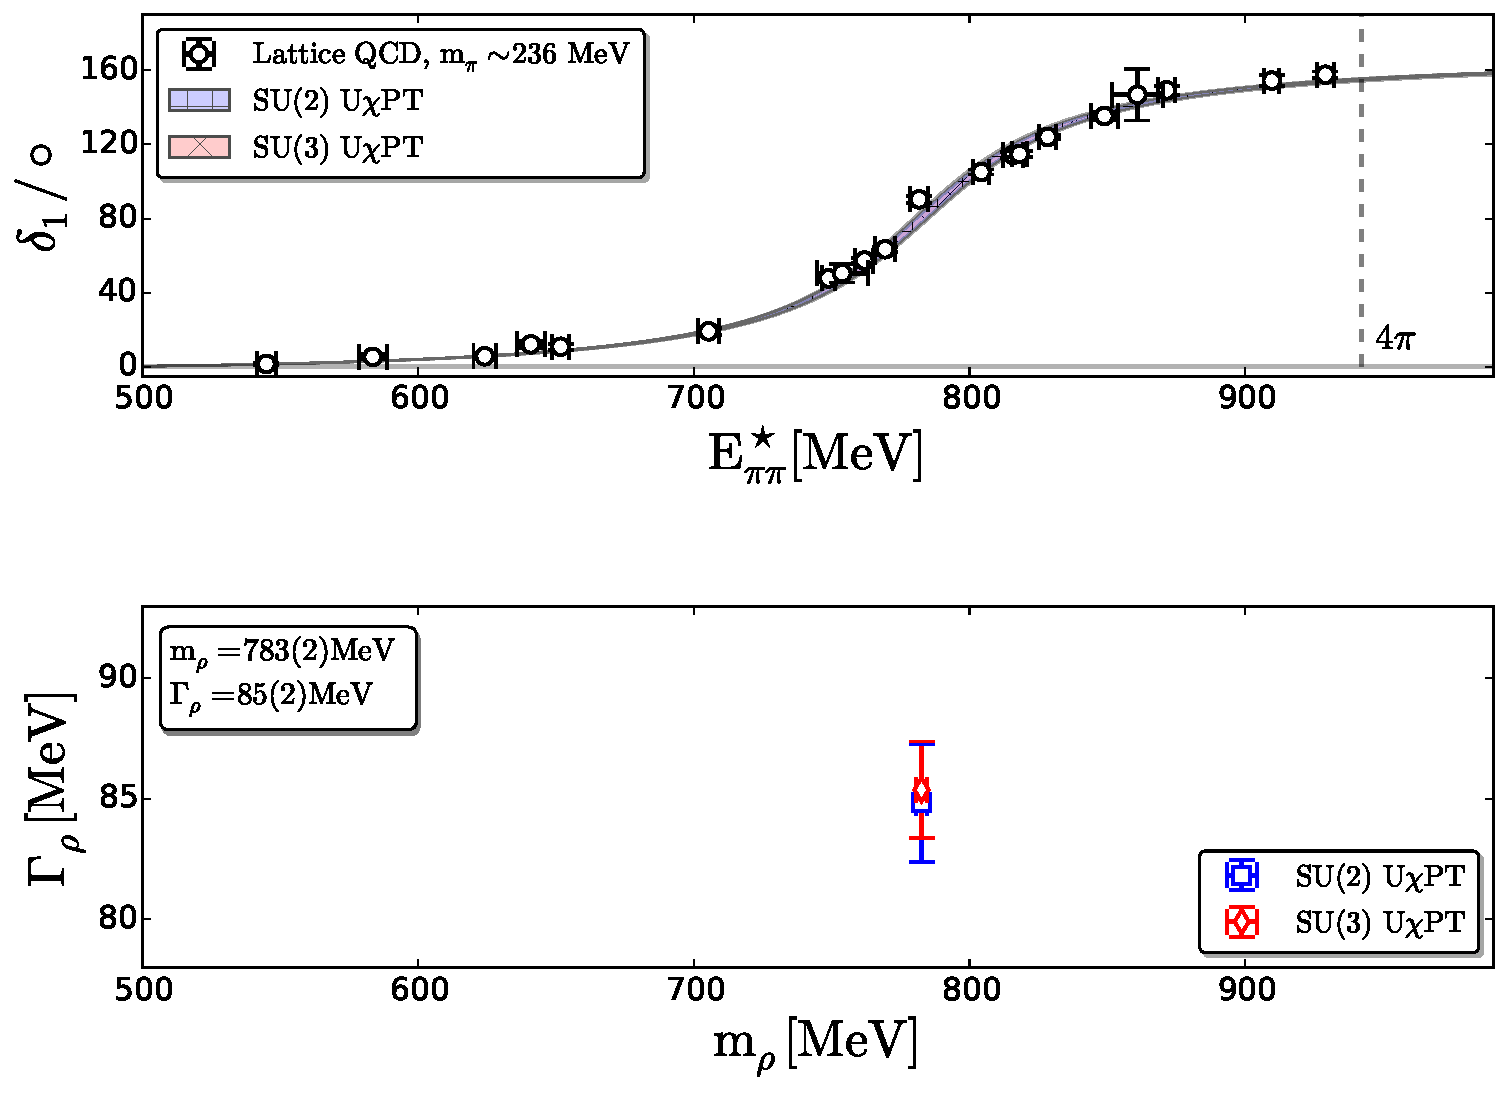
\includegraphics[scale=0.35]{figures/lattice_fits.pdf}
%generated in rho_860/lattice_fits.py
\caption{The upper panel shows the $I=1$ $\pi\pi$ phase shift obtained from the lattice QCD spectrum determined at $m_\pi\approx236$~MeV as a function of the c.m. energy. The dashed line shows the $4\pi$ threshold. Also shown are the SU(2) and SU(3) U$\chi$PT fits. One observes that these two results are indistinguishable at these quark masses. The lower panel shows the mass of the $\rho$ pole ($m_\rho\equiv\rm Re(E_\rho)$) along with its width ($\Gamma_\rho\equiv\rm 2 Im(E_\rho)$). We do not show two noisy energy levels.
}
\label{fig:lattice_fits}
\vspace*{-.6cm}
\end{center}
\end{figure}
%%%%%%%%%%%%%%%%%%%%%%%%%%%

In calculating the amplitude at $m_\pi\approx 236$~MeV, we use the meson masses determined by lattice QCD. For $f_\pi$ we use the NLO $\chi$PT expression~\cite{Gasser:1984gg,Gasser:1983yg,Gasser:1983kx}
\begin{align}
f_\pi(m_\pi)=f_0\left(1-\frac{1}{16\pi^2}\frac{m_\pi^2}{f_\pi^2}\ln\frac{m_\pi^2}{\mu^2}+\ell_4(\mu)\right)
\end{align}
where $\mu$ is the renormalization scale. We define $f_0$ such that the right hand side coincides with the physical value of the decay constant.  

To perform a chiral extrapolation we must determine the lattice spacing. We use two definitions of the lattice spacing. First, we use the $\Omega$ baryon mass, which has been determined to be $a_tm_\Omega^{\rm latt.}=0.2789(16)$ at these quark masses~\cite{Wilson:2015dqa}. By setting this equal to $a_tm_\Omega^{\rm phys.}$ ($m_\Omega^{\rm phys.}=1672.45(29)~\rm MeV$ is the mass of physical $\Omega$ baryon) we obtain the lattice spacing $\rm a_t^{[1]}=0.1668(10)~GeV^{-1}$.  Second, we perform a chiral extrapolation of the lattice $\Omega$ baryon mass using $m_\Omega(m_\pi)=m_{\Omega,0}+\alpha m_\pi^2+\beta m_\pi^4$ determined for four different values of $m_\pi/m_\Omega\in[0.14-0.33]$ \cite{Lin:2008pr, Wilson:2015dqa}. We find $\rm a^{[2]}_t=0.1630(14)~GeV^{-1}$ with a $\rm \chi^2/d.o.f.=0.52$. Given that $\rm a_t^{[1]}$ should coincide with $\rm a_t^{[2]}$, we perform all fits using both of these lattice spacings and any deviation of the result is incorporated into the systematic error. All central values below are obtained using the mean value of $\rm a_t^{[1]}$. As is shown below, this $2\%$ error is the largest source of uncertainty in our final result. This systematic error is improvable.

%%%%%%%%%%%%%%%%%%%%%%%%%%%
\begin{figure}[b]
\begin{center}
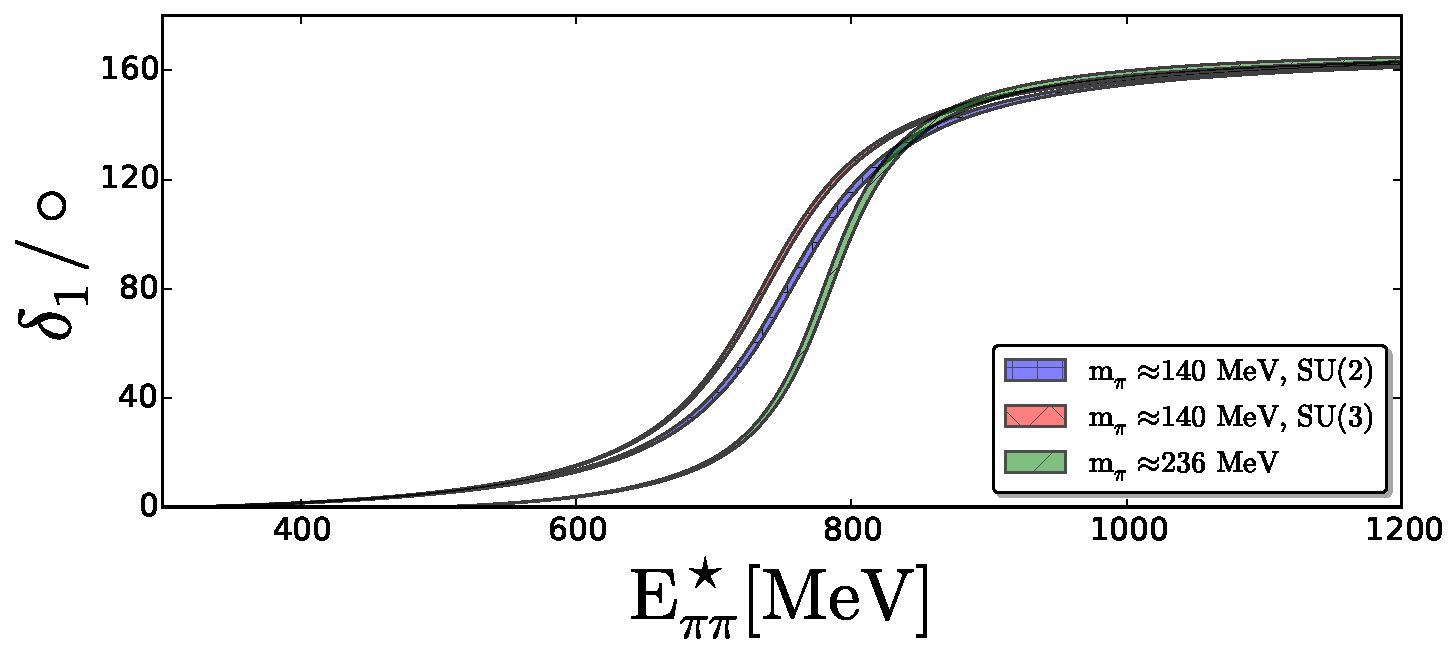
\includegraphics[scale=0.35]{figures/SU2_SU3_comparison.pdf}
%%%%%generated in rho_860/SU2_3_comparison.py
\caption{Shown is the $I=1$ $\pi\pi$ phase shift as a function of the c.m. energy determined at $m_\pi\approx 236$~MeV (green) compared with the extrapolated phase shift using SU(2) and SU(3) in blue and red respectively. These results use $\rm a_t=0.1668~GeV^{-1}$ and the bands indicate the statistical uncertainty. For the systematic uncertainty due to the lattice spacing see Fig.~\ref{fig:global_comparison}. }
\label{fig:extrapolations}
\vspace*{-.6cm}
\end{center}
\end{figure}
%%%%%%%%%%%%%%%%%%%%%%%%%%%
 
%%%%%%%%%%%%%%%%%%%%%%%%%%%
\begin{figure*}[t]
\begin{center}
\hspace*{-.7cm}                                                           
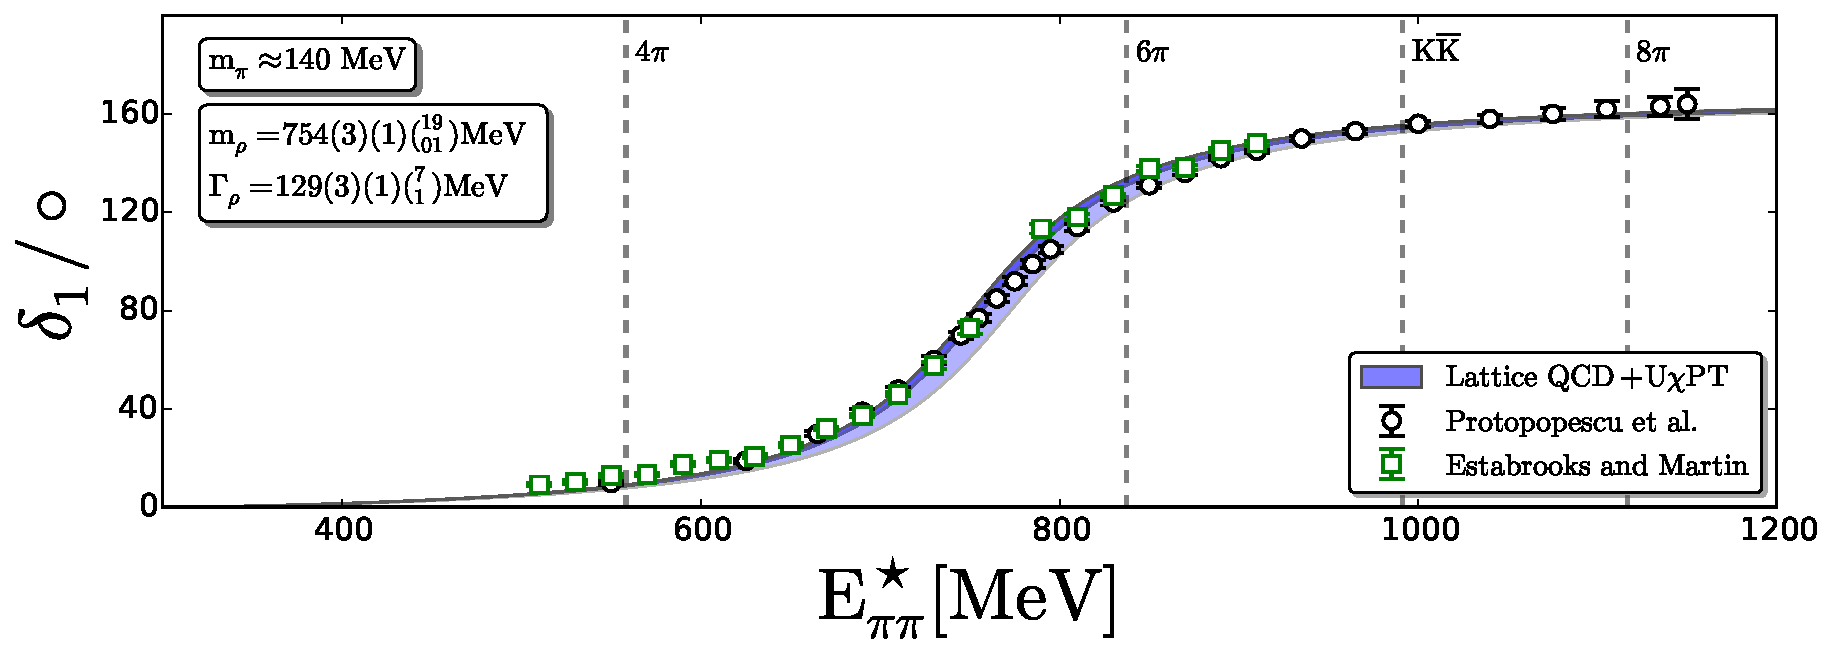
\includegraphics[scale=0.59]{figures/global_comparison.pdf}
%generated in rho_860/lattice_vs_exp.py
\caption{Shown is the extrapolated $\pi\pi$ $\ell=1$ scattering phase shift as a function of the c.m. energy $(\rm E^\star_{\pi\pi})$. The darker blue inner band includes only statistical uncertainty, while the lighter outer band also includes systematic uncertainty. We see good agreement with the experimental phase shift shown as black circles~\cite{Protopopescu:1973sh} and green squares~\cite{Estabrooks:1974vu}. The dashed line denote the $4\pi$, $6\pi$, $K\overline{K}$ and $8\pi$ thresholds, which seem to play a negligible role. }\label{fig:global_comparison}
\end{center}
\vspace*{-.6cm}
\end{figure*}
%%%%%%%%%%%%%%%%%%%%%%%%%%%

 

%This has been determined using different techniques. This has, for example, been estimated in Ref.~\cite{Lin:2008pr} by extrapolating the $\Omega$ baryon mass to the physical point to be $a_t = 0.03506(23)$~fm.  

Having 22 energy levels at a single quark mass and spatial volume, we are able to fit the two unknown low-energy coefficients. The fit results in $\chi^2/ N_\mathrm{d.o.f.} = 1.26/1.19 $ for SU(2) and SU(3) U$\chi$PT respectively and is shown in Fig.~\ref{fig:lattice_fits} compared to the lattice determined phase shifts. The phase shift is plotted as a function of the c.m. $\pi\pi$ energy, $\rm E^\star_{\pi\pi}$. The SU(2) low-energy coefficients and correlations are found to be

\begin{center}
\begin{tabular}{rll}
$\alpha_1(770~\rm MeV)=$                         & $ 14.7(4)(2)(1)\times~10^{-3} $   & 
\multirow{2}{*}{ $\begin{bmatrix*}[r] 1 &  -0.95   \\ 
                                    			&  1   \\ \end{bmatrix*}$ } \\
$\alpha_2(770~\rm MeV) =$                 & $-28(6)(3)(^{01}_{11})\times~10^{-3}$   & \\
%&\multicolumn{2}{l}{ $\chi^2/ N_\mathrm{d.o.f.} = \frac{25.15}{22-2} = 1.26 $\,.}
\end{tabular}~~~~
\end{center}
\vspace{-1cm}
\begin{equation} \label{eq:lecs}\end{equation}
The first uncertainty is statistical, the second is the systematic due to the determination of the $\pi$ mass and the anisotropy of the lattice~\footnote{The $\pi$ mass was determined in lattice units to be $a_tm_\pi=0.03928(18)$. The anisotropy of that lattice is defined as $\xi=a_s/a_t$ where $a_s$ and $a_t$ are the lattice spacings in the spatial and temporal extents. The anisotropy has been determined to be $\xi=3.4534(61)$.}, and the third is an estimate of the systematic due to the determination of the lattice spacing. The matrix on the right of the coefficients denotes the statistical correlation between the two. 
By analytically continuing the scattering amplitude to the complex plane we obtain the resonance pole at these quark masses $E_\rho=783(2)-i\,43(1)$~MeV. From the imaginary piece of the pole we obtain the width of the $\rho$, $\Gamma_\rho\equiv\rm 2 Im(E_\rho)=85(2)$~MeV. We observe good agreement with the result by the Hadron Spectrum collaboration where the poles were determined using other parametrizations of the scattering amplitude. This emphasizes the fact that the lattice QCD spectrum properly constrains the scattering phase shift, independent of the parametrization chosen. 

 
This result holds not just at the quark masses used for the lattice QCD calculation. The power of the U$\chi$PT amplitude is that it allows one to analytically continue these quantities to the physical point as well as other values of the quark masses. In Fig.~\ref{fig:extrapolations} we show the result of this exercise using $\rm a_t=0.1668~GeV^{-1}$ for both SU(2) and SU(3) U$\chi$PT. It is evident that despite there being a slight deviation between the SU(2) and SU(3) statistical bands, both of these extrapolations closely resemble the experimental determination of the $\pi\pi$ phase shift. Due to large SU(3) breaking effects in the range of quark masses considered, SU(3) $\chi$PT has poorer perturbative convergence and the systematic errors associated with higher order corrections in the chiral expansion are difficult to properly asses. 

In Fig.~\ref{fig:global_comparison} we present our final result for the chiral extrapolation of the $\pi\pi$ phase shift using SU(2) U$\chi$PT. The result include a propagation of statistical and systematic uncertainties. The largest uncertainty is due to the determination of the lattice spacing, where we have been rather conservative. Overall, we find remarkably good agreement with the experimental phase shift~\cite{Protopopescu:1973sh, Estabrooks:1974vu} up to center of mass energies of 1.2~GeV, well above the $4\pi$, $6\pi$, $K\overline{K}$ and $8\pi$ thresholds. By analytically continuing the amplitude into the complex plane, we find a \emph{postdiction} of the $\rho$ pole at the physical point $E_\rho=\Erho$.  
  

\emph{Final remarks:} We present the first chiral extrapolation of a resonant phase shift. Unlike prior chiral extrapolations of the $\rho$ resonance~\cite{Leinweber:2001ac, Feng:2010es}, we do not rely on effective field theories where the $\rho$ is treated as an asymptotic degree of freedom whose unstable nature only emerges as an aftereffect of coupling this state onto $\pi\pi$ states~\footnote{Such effective field theories are perfectly sound, as they introduce an integrable auxiliary field via a field transformation.}. Instead we used U$\chi$PT, an effective field theory that at low-energies coincides with $\chi$PT and at high-energies generates resonances dynamically. In this framework, resonances are manifested naturally as singularities in amplitudes. We observe that this effective field theory does a remarkable job in describing the recent results of the Hadron Spectrum Collaboration. Using only the lattice QCD spectrum to fit the low-energy coefficients of the theory, we find great agreement with the experimental determination of the $\pi\pi$ scattering phase shift up to energies above the $8\pi$ and $K\overline{K}$ thresholds illustrating the significance of this result. 

Looking to the future one can foresee the study of more complex systems such as highly energetic exotic hadrons (e.g., the $\pi_1(1400)$ resonance) or heavy meson weak decays (e.g., $D\rightarrow \pi\pi/K\overline{K}$ \cite{Hansen:2012tf, Aaij:2011in}). Although it is not yet clear when a finite volume formalism rigorously accommodating all open channels will be available, one can envision making controlled chiral extrapolations of these quantities regardless of their resonant content. We demonstrate that by properly constraining the scattering amplitude at one value of the $\pi$ mass one can, in principle, perform such extrapolations.

In this work we restricted our analysis to the $I=1$ $\pi\pi$ channel with $m_\pi\approx236$~MeV. There is a wealth of available results at $m_\pi\approx 400$~MeV~\cite{Dudek:2012xn, Dudek:2010ew, Dudek:2012gj, Dudek:2014qha, Wilson:2014cna} that will be analyzed in the near future using the techniques presented here. These studies will help asses the systematic errors of SU(2) and SU(3) U$\chi$PT. These techniques are expected to have a major impact not just in the determination of the spectrum from QCD, but also in the determination of transition amplitudes.
 
 {\raul [I am not totally happy with the conclusion...]}


 %%%%%%%%%%%%%%%%%%%%%%%%%%%%%%%%%%%%%%%%%%%%
\subsection*{Acknowledgments}


D.B. would like to thank Jacob Emerick, Chris Madrid, and Keith Robertson for their help with this project. R.B. acknowledges support from the U.S. Department of Energy contract DE-AC05-06OR23177, under which Jefferson Science Associates, LLC, manages and operates the Jefferson Lab. We would like to thank our colleagues in the Hadron Spectrum Collaboration, in particular {\raul J. Dudek,  Robert G. E. and C.~E.~Thomas}, for granting us permission to analyze the recent results of the Hadron Spectrum Collaboration and for useful discussions and feedback on the manuscript. 



 %%%%%%%%%%%%%%%%%%%%%%%%%%%%%%%%%%%%%%%%%%%%%%%%%%%%%%%%%%%%%%%%%
%%%%%%%%%%%%%%%%%%%%%%%%%%%%%%%%%%%%%%%%%%%%%%%%%%%%%%%%%%%%%%%%%

%%%%%%%%%%%%%%%%%%%%%%%%%%%%%%%%%%%%%%%%%%%%%%%%%%%%
 
\bibliography{bibi}






 %%%%%%%%%%%%%%%%%%%%%%%%%%%%%%%%%%%%%%%%%%%%%%%%%%
\end{document}

